\documentclass[11pt]{article}


%opening

%%% PACKAGES
\usepackage[english]{babel}
\usepackage[T1]{fontenc} % pouzije EC fonty
\usepackage[utf8]{inputenc} % set input encoding (not needed with XeLaTeX) 
\usepackage{booktabs} % for much better looking tables
\usepackage{array} % for better arrays (eg matrices) in maths
\usepackage{paralist} % very flexible & customisable lists (eg. enumerate/itemize, etc.)
\usepackage{verbatim} % adds environment for commenting out blocks of text & for better verbatim
\usepackage{subfigure} % make it possible to include more than one captioned figure/table in a single float
\usepackage{color}
\usepackage{xcolor}
\usepackage{listings}
\lstset{
	frame=top,frame=bottom,
	basicstyle=\small\normalfont\sffamily,    % the size of the fonts that are used for the code
	stepnumber=1,                           % the step between two line-numbers. If it is 1 each line will be numbered
	numbersep=10pt,                         % how far the line-numbers are from the code
	tabsize=2,                              % tab size in blank spaces
	extendedchars=true,                     %
	breaklines=true,                        % sets automatic line breaking
	captionpos=t,                           % sets the caption-position to top
	mathescape=true,
	stringstyle=\color{blue}\ttfamily, % Farbe der String
	keywordstyle=\color{blue}\ttfamily,
	commentstyle=\color{green}\ttfamily,
	showspaces=false,           % Leerzeichen anzeigen ?
	showtabs=false,             % Tabs anzeigen ?
	xleftmargin=17pt,
	framexleftmargin=17pt,
	framexrightmargin=17pt,
	framexbottommargin=5pt,
	framextopmargin=5pt,
	showstringspaces=false      % Leerzeichen in Strings anzeigen ?
}

\usepackage{caption}

%\usepackage[demo]{graphicx}

%\usepackage{pdfpages}


% Potřeba pro matematické vzorec a align
\usepackage{amsmath}
\usepackage{graphicx} % support the \includegraphics command and options
\usepackage{geometry}
\geometry{left=1in, right=1in}

\numberwithin{equation}{section}

\title{ROVI - Exercise 2}
\author{Petr Batek, Bjarki Páll Sigurðsson}


\begin{document}
\selectlanguage{english}

\maketitle

\newpage

\section{Introduction}
Purpose of this exercise was to get familiar with working with Robwork libraries and use simple planning algorithm RRT in our C++ project. We used provided template \texttt{pathplanning.cpp} as a starting point for our implementation. We extended template file with several functions. One is for creating a Lua file, which is used for animations in Robwork studio. Another function was written for creation of file with results from numerous simulations. These results were used further in order to find reasonable value for $\epsilon$, which is the smallest step in radians for joints of robot manipulator.

\section{C++ and Lua file}
It was important to grab the bottle frame before we started path planner algorithm. This was done by commands shown on listing \ref{lst::gripFrame}.


\begin{lstlisting}[caption={Grabbing Bottle frame into Gripper}, language=C++, label={lst::gripFrame}]
// Finds the frame of gripper
const string gripperName = "Tool";
rw::kinematics::Frame *gripper = wc->findFrame(gripperName);

// Finds the frame of Bottle
const string itemName = "Bottle";
rw::kinematics::MovableFrame *item;
item = (MovableFrame *) wc->findFrame(itemName);

// Loads inital state of the scene
State state = wc->getDefaultState();
// Before Grapping the Bottle, manipulator must be se to correct possition
device->setQ(from, state);
// When Manip. is in correct possition, it can grip the frame
Kinematics::gripFrame(item, gripper, state);


\end{lstlisting}

We used provided \texttt{Lua} file as a template for creating animation scripts. In our function \texttt{createLuaFile} we first copy the first part of the script. After that there are inserted commands for setting of joints coordinates to values computed by C++ program. Finally the ending part of template is copied to new \texttt{Lua} file.

\newpage
\section{Chossing of $\epsilon$ value}
To find reasonable $\epsilon$ value we had run several simulations, which statistics were finally compared. We selected a grid of different $\epsilon$ values and for each of them run 1000 of simulations. We set random seed for random number generator in order to receive different results for each simulation. 

Histograms for 5 different values of $\epsilon$ are plotted on Figure \ref{fig::histograms}. It can be seen that Computation Time and No. of Nodes are seriously affected by the value of $\epsilon$. On the other hand total path length isn't affected in such a large scale.
\begin{figure}[h]
	\centering
	\hspace*{-2cm}
	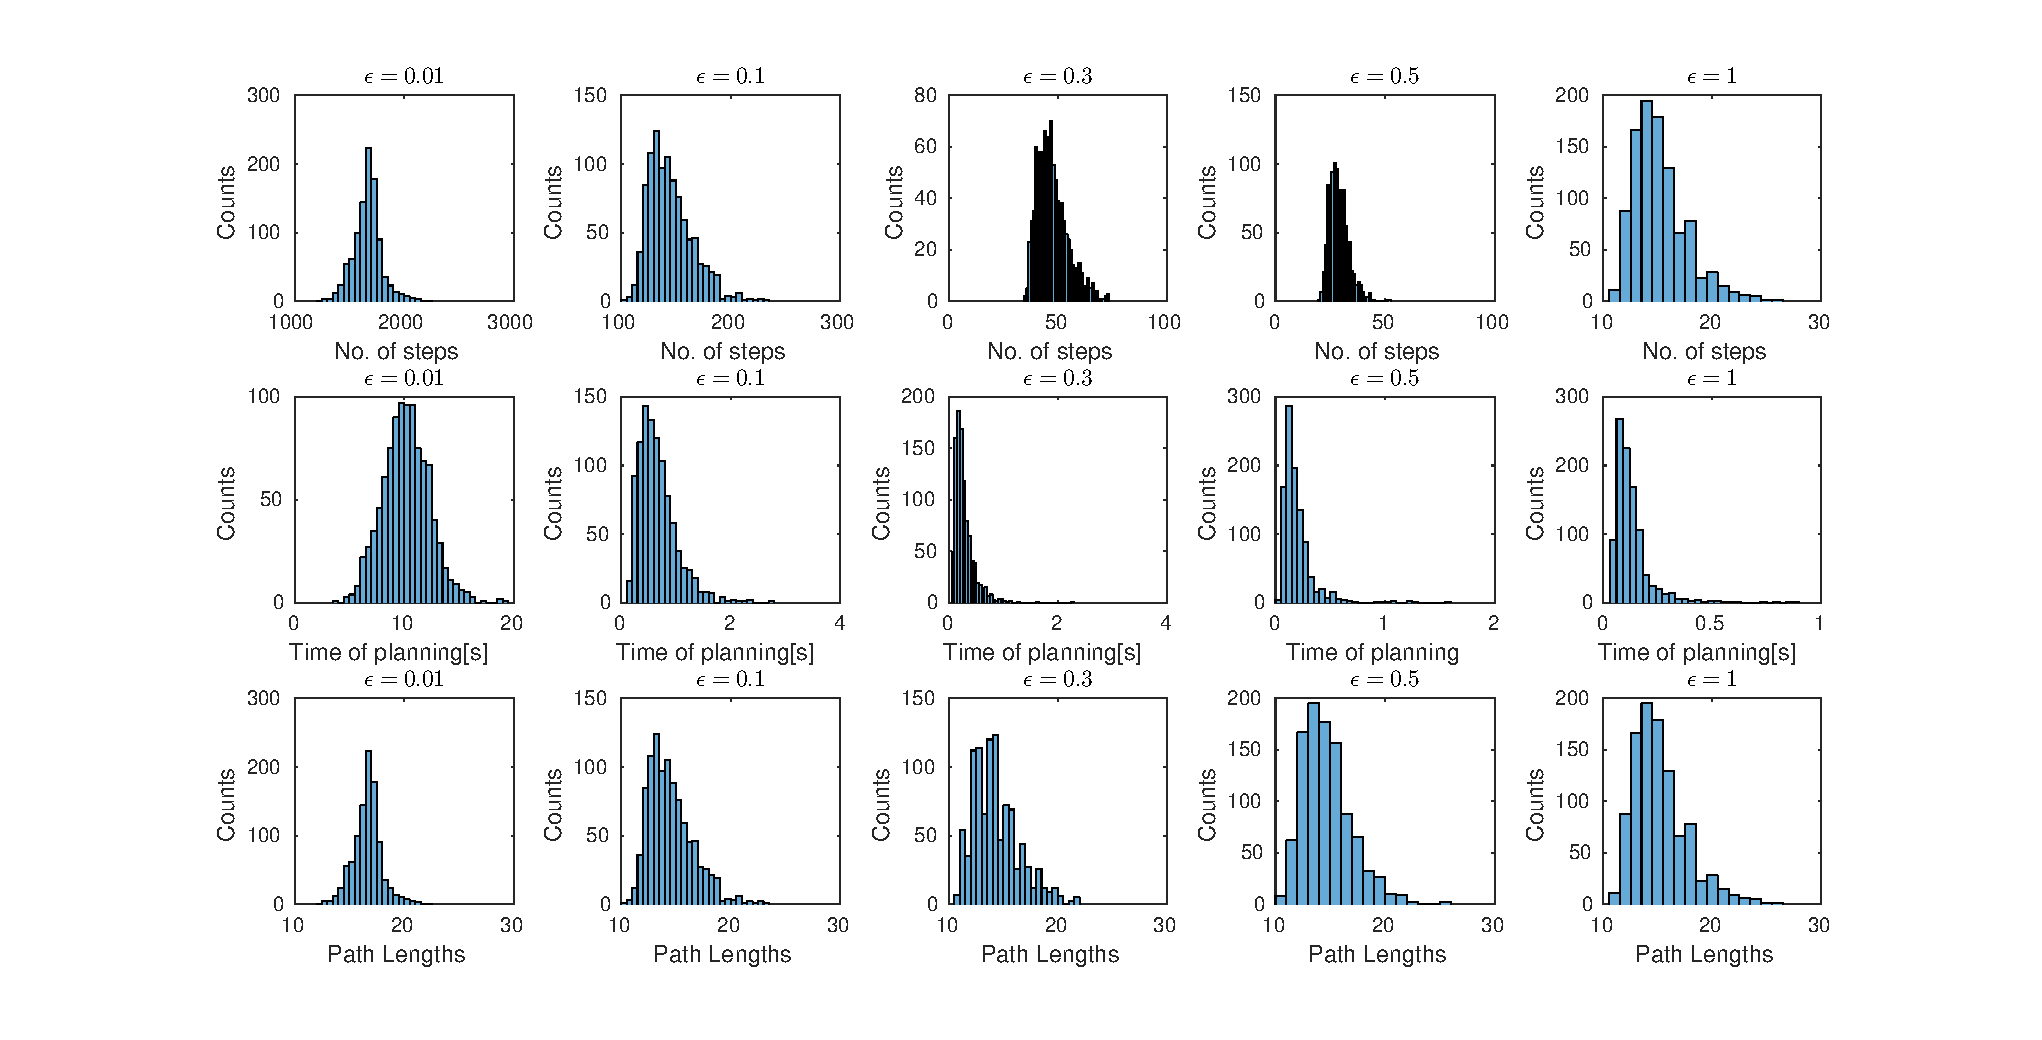
\includegraphics[width = 20cm]{fig/Histograms.eps}
	\caption{Histograms of simulations results}
	\label{fig::histograms}
\end{figure}

Mean values of simulation results were computed after that. We compared these parameters:

\begin{itemize}
	\item average Number of Nodes = number of joints configurations before reaching the goal state
	\item average Computation time
	\item average Path Length = average total distance in joints coordinate frame, computed according equation:
	$$ Path Length\; =\; \#\, of\, Nodes\, \cdot \, \epsilon$$
\end{itemize} 

There are results on the Figure \ref{fig:comparison}. It is apparent that average computation time is decreasing for larger $\epsilon$ values. In contrast, Average Path Lenght isn't a monotone function. There is a minimum for value $\epsilon = 0.2$. It seems that this is our reasonable value. 
\begin{figure}[h]
	\centering
	\subfigure[Average Computation Time]{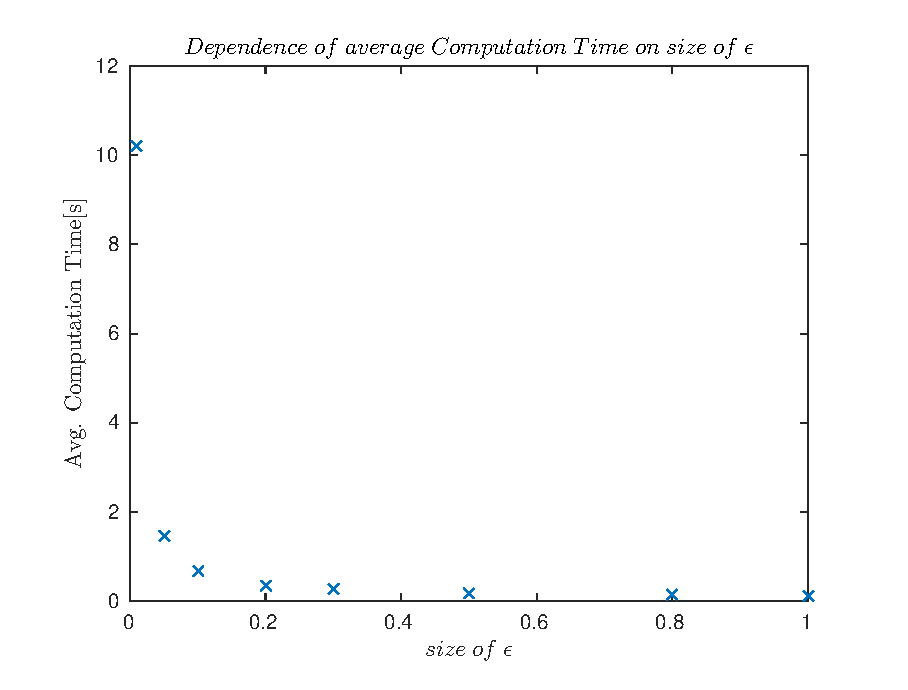
\includegraphics[width=8cm]{fig/AvgCompTime.eps}}
	\hfill
	\subfigure[Average Path length]{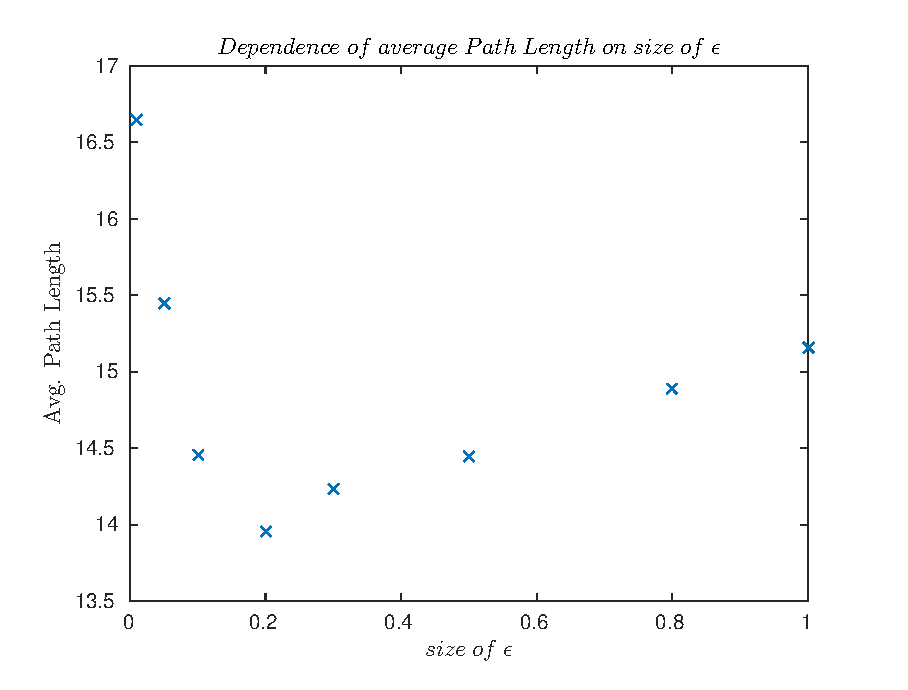
\includegraphics[width=8cm]{fig/AvgPathLen.eps}}
	\hfill
	\caption{Comparison of different Computation Time and Path Lengths for $\epsilon$ parameter}
	\label{fig:comparison}
\end{figure} 

For another point of view we plotted a comparison of Average Path Length versus Average Computation Time into a single graph. It is plotted on Figure \ref{fig::avepathlenvsavecomptime}. This plot offers new insights into our problem. The closer is the point to the origin, the better performance regarding computation time and path length. This insight confirms, that value of $\epsilon = 0.2$ is suitable for our problem. From this graph it is also possible to predict, that any value in interval $\epsilon \in \left[0.1,\,0.5\right]$ will result in short path with low computation time. $\epsilon$ with values $0.8$ and $ 1$ also results in low computation time, however the path length is considerable larger. If we consider parameter values lower than $0.1$, it can be seen that they are worse in both aspects, longer computation time and total path length. 

\begin{figure}[h]
	\centering
	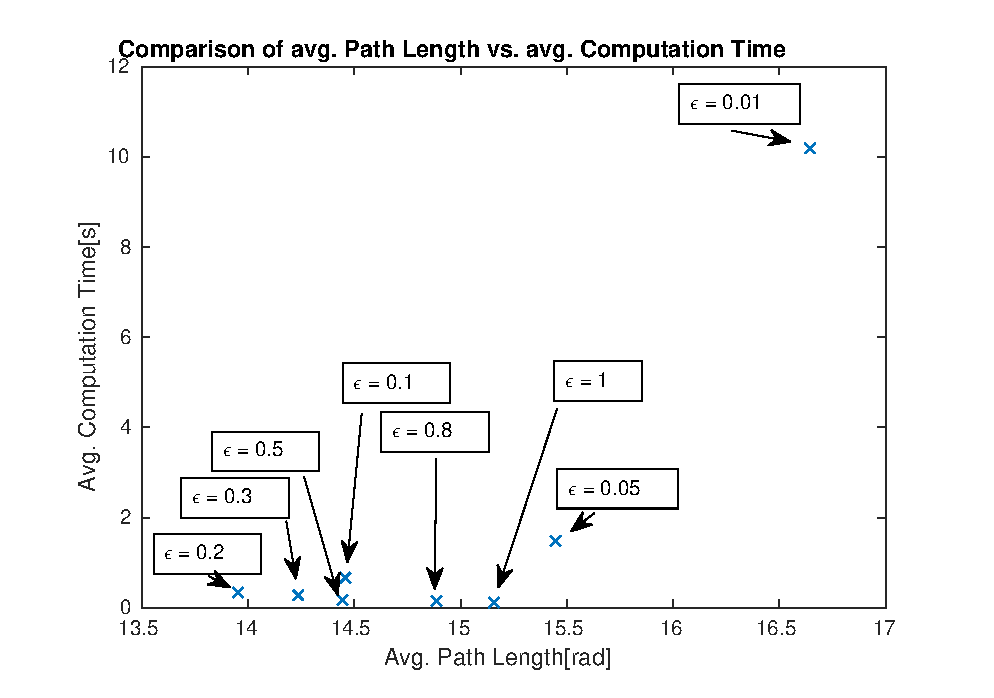
\includegraphics[width = 16cm]{fig/PathVsTime.eps}
	\caption{Average Path Length versus Average Computation Time}
	\label{fig::avepathlenvsavecomptime}
\end{figure}

\section{Conclusion}
In this exercise we used Robwork RRT path planning method to find path for transfer object from start point to end point. We got familiar with Lua script used for animations in Robwork studio. We have found reasonable value for path planner parametr $\epsilon$ after performation of statistical tests. In order to find optimal $\epsilon$ value with respect to Computation time and Path length, it would be possible to create a finer grid of $\epsilon$ values and run statistical tests for each of them. Nevertheless we consider value of $\epsilon = 0.2$ as good enough.




\end{document}
